\documentclass[../diplomski_rad.tex]{subfiles}

\begin{document}

\sloppy

\justifying

shema sustava i za sto je

\section{STM32WB5MMG bežični modul}

STM32WB5MMG bežični modul predstavlja kompaktno i visoko integrirano rješenje za razvoj pametnih uređaja koji zahtijevaju bežičnu povezanost. 
Baziran je na mikrokontroleru STM32WB55VGY te pruža mogućnost Bluetooth Low Energy i Zigbee bežične komunikacije. 
U modul je integrirana antena i kvarcni oscilatori što znatno olakšava i ubrzava razvoj sklopovlja.  

\begin{figure}[htb]
    \centering
    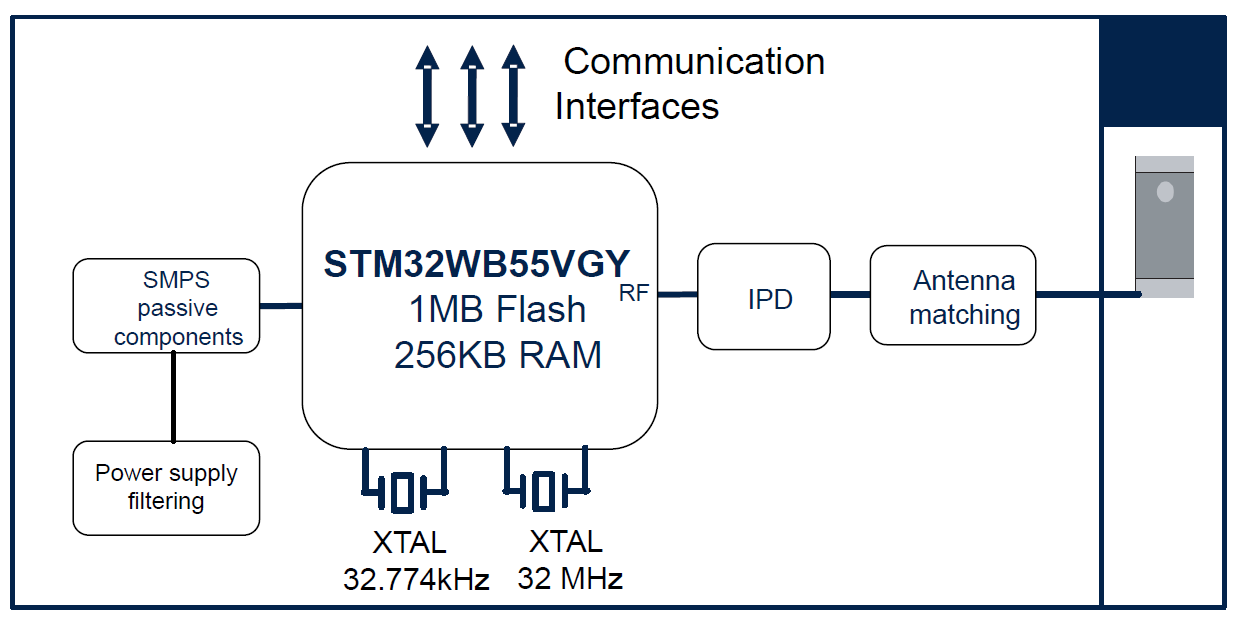
\includegraphics[width=0.75\textwidth]{Figures/stm32module.png} 
    \caption{Block shema STM32WB5MMG modula \cite{stm32module}}
    \label{slk:stm32module}
\end{figure}

Modul dolazi u LGA kućištu veličine 7.3x11 milimetara. Iz blok sheme modula, prikazane na slici \ref{slk:stm32module}, 
vidljivo je kako se modul sastoji od:
\begin{itemize}
    \item STM32WB55VGY mikrokontrolera,
    \item antene,
    \item niskofrekvencijskog kvarcnog oscilatora frekvencije 32.768 kHz,
    \item visokofrekvencijskog kvarcnog oscilatora frekvencije 32 MHz,
    \item Pasivne komponente za SMPS (engl. \textit{switched-mode power supply}) 
    \item Integrirane pasivne komponente (IPD) za uklanjanje harmonika i usklađivanje RF impedancije.     
  \end{itemize} 
Zbog niske potrošnje, visokog stupnja integriranosti i malih dimenzija pogodan je za razvoj nosivih uređaja, 
čija je glavna karakteristika da moraju biti bežično povezani sa drugim uređajima. 

- slika kucista mozda?

\subsection{STM32WB55VGY mikrokontroler}

STM32WB55VGY je dvojezgreni mikrokontroler s ugrađenom podrškom za bežičnu komunikaciju. 
To je sistem na čipu koji unutar jednog čipa integrira mikrokontroler opće namjene i mrežnu funcionalnost. 
Sastoji se od dvije jezgre, ARM Cortex-M4 te ARM Cortex-M0+.  
ARM Cortex-M4 jezgra izvršava aplikacijski kod te radi na maksimalnoj frekvenciji od 64 MHz. 
Mrežni procesor ARM Cortex-M0+ zadužen je za upravljanje bežičnim komunikacijskim protokolima 
te potpuno neovisno od aplikacijske jezgre održava bežičnu vezu.
Jezgre međusobno komuniciraju pomoću međuprocesorskog komunikacijskog kontrolera (engl. \textit{IPCC,  Inter Processor
Communication Controller}). 
Dijeljenje resursa među jezgrama kontrolirano je sklopovskim semaforima.

\begin{figure}[htb!]
    \centering
    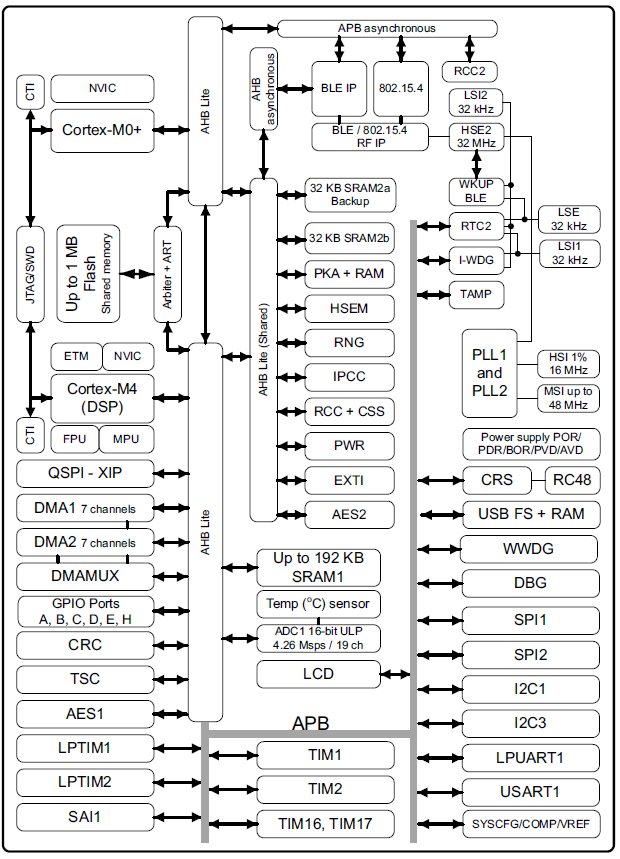
\includegraphics[width=0.6\textwidth]{Figures/stm32mikro.png} 
    \caption{Block shema STM32WB55VGY mikrokontrolera \cite{stm32mikro}}
    \label{slk:stm32mikro}
\end{figure}

Mikrokontroler ima 1MB flash memorije, 256kB SRAM memorije te sve uobičajne periferije za mikrokontrolere opće namjene. 
Na slici \ref{slk:stm32mikro} prikazana je blok shema mikrokontrolera na kojoj su vidljive sve dostupne periferije.
Razvoj programske potpore za korišteni mikrokontroler opisan je u poglavlju (\ref{chap:programska_podrska}).

\section{Senzori}

Senzori su ključan dio razvijenog nosivog sustava jer omogućuju kontinuirano praćenje podataka potrebnih 
za dijagnostiku i praćenje zdravstvenog stanja pacijenata u stvarnom vremenu.
U daljnjem tekstu dan je detaljan pregled svih korištenih senzora razvijenog sustava.

\subsection{Senzor inercije}

Senzor ICM-20948 koristi se za mjerenje inercije te pruža precizno praćenje kretanja i orijentacije u prostoru.
Unutar jednog čipa ima integriran akcelerometar, žiroskop i magnetometar što pruža sveobuhvatnu sliku o kretanju 
i položaju objekta u trodiomenzionalnom prostoru. 

- treba li tu sto detaljnije (komunikacjski protokoli, konkretne karakteristike..)?

\begin{figure}[htb]
    \centering
    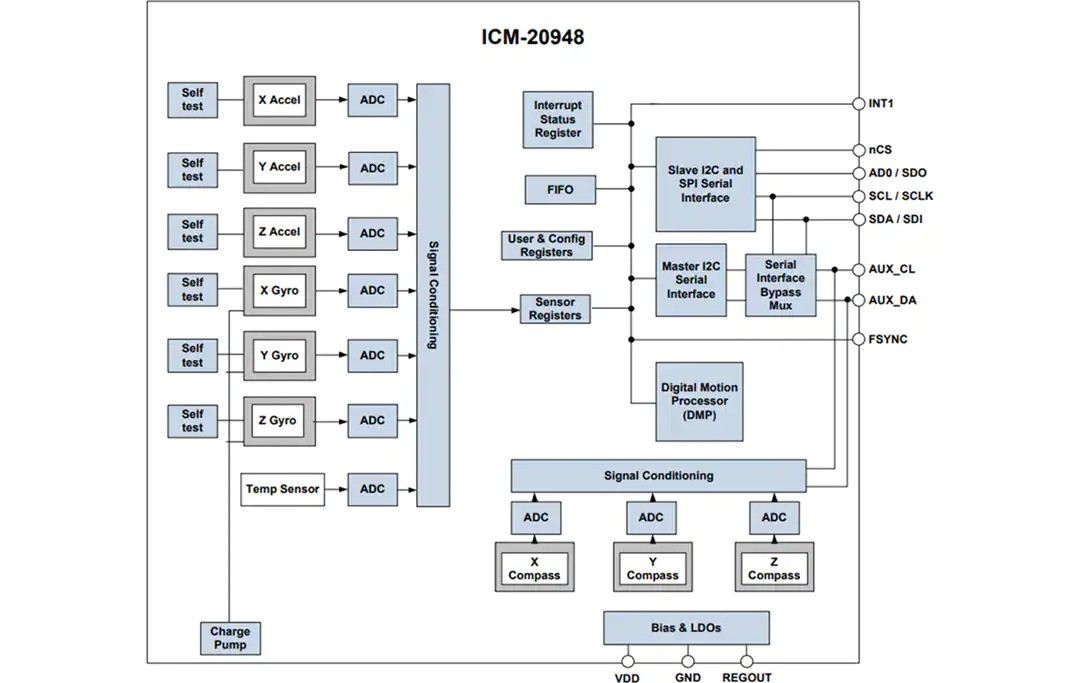
\includegraphics[width=0.75\textwidth]{Figures/ICM-20948.jpg} 
    \caption{Block shema senzora ICM-20948 \cite{icm20948}}
    \label{slk:icm20948}
\end{figure}

Senzor komunicira s ostatkom sustava pomoću I2C ili SPI komunikacije te na zahtjev šalje mikrokontroleru tražene podatke.
Važno je naglasiti da je ICM-20948 dizajniran s naglaskom na energetsku učinkovitost i malu potrošnju energije 
što ga čini dobrim izborom za nosive uređaje.

\subsection{Integrirano sučelje za mjerenje bioimpedancije}

MAX30009 je integrirano sučelje za mjerenje bioimpedancije dizajnirano za primjene u nosivim tehnologijama. 
Izrazito je male potrošnje (250 $\mu$W na napajanju od 1.8 V)\cite{max30009} i malih dimenzija (2.03x2.03 mm) što ga čini idealnim izborom za bežični nosivi uređaj.  

Senzor radi na principu puštanja male sinusne struje kroz tijelo i mjerenjem pada napona kroz tijelo. 
U sebi ima integrirani generator pobudne sinusne struje u širokom rasponu frekvencija i jakosti struja. 
Raspon frekvencija je od 16 Hz do 500 kHz, a jakosti struja od 16nA\textsubscript{RMS} do 1.28mA\textsubscript{RMS} \cite{max30009}.

Ulazni priključci elektroda spojedni su na multipleksore čime se dobiva mogućnost izbora 
između različitih setova elektroda. Također senzor podržava dvožično kao i četverožično mjerenje bioimpedancije.

MAX30009 pruža kalibracijski priključak za vanjski četverožičani precizni referentni otpor koji se koristi tijekom kalibracije. 
Također, dostupni su i interni otpornici koji se mogu koristit za kalibraciju, ali uz manju točnost od vanjskog referentnog otpornika.
Kalibracija je potrebna prilikom korištenja MAX30009 za bioimpedancijska mjerenja koja zahtijevaju apsolutnu točnost poput BIA i BIS mjerenja.

-konkretno o mjernom kanalu unutra?
-reference na datasheet?

\subsection{AD4950}

\end{document}